\documentclass[11pt,letterpaper]{article}

%% ---- Packages ----
\usepackage[utf8]{inputenc}
\usepackage[T1]{fontenc}
\usepackage{mathpazo}
\usepackage[margin=2cm]{geometry}
\usepackage{graphicx}
\usepackage{float}
\usepackage{caption}
%% labelfont=bf + labelsep=period make the AUTO-generated label render as
%% "\textbf{Extended Data Fig. 7.}", which is byte-for-byte what the hand-written prefix inside
%% each \caption used to produce. The prefix has been removed from all seven captions; keeping
%% both printed "Extended Data Fig. 7: Extended Data Fig. 7." on every figure. Numbering is now
%% the counter's, so a caption can no longer disagree with its own \label.
\captionsetup{singlelinecheck=false, font={small}, skip=4pt, labelfont=bf, labelsep=period}
\usepackage{amsmath,amssymb}
\usepackage{booktabs}
\usepackage[dvipsnames]{xcolor}
\usepackage[most]{tcolorbox}
\usepackage{hyperref}
\usepackage[numbers,sort&compress,super]{natbib}
\usepackage{enumitem}
\usepackage{lineno}
\linenumbers
%% Same value as the main manuscript (seed-resampling control range).
\newcommand{\CONTROLRANGE}{1 to 4}
\newcommand{\TODO}[1]{{\color{BrickRed}\textbf{[[#1]]}}}

%% ---- Section formatting (Nature Methods style) ----
\usepackage{titlesec}
\titleformat{\section}{\large\bfseries}{}{0em}{}
\titleformat{\subsection}{\normalsize\bfseries}{}{0em}{}
\titlespacing*{\section}{0pt}{1.5ex plus 0.5ex}{0.8ex plus 0.2ex}
\titlespacing*{\subsection}{0pt}{1.2ex plus 0.3ex}{0.5ex plus 0.1ex}

\hypersetup{colorlinks=true,linkcolor=MidnightBlue,citecolor=MidnightBlue,urlcolor=MidnightBlue}
\setlength{\emergencystretch}{3em}

\title{Supplementary Information: Objective-aligned evaluation inflates distributional gains in single-cell drug retrieval}
\author{\TODO{Author list, as in the main manuscript}}
\date{}
\renewcommand{\figurename}{Extended Data Fig.}
\begin{document}
\maketitle
\noindent This Supplementary Information contains seven Extended Data figures, four Supplementary
Notes, and four Supplementary Tables. Supplementary Note 4, which states the scope of every
claim in the paper, is the last item in this document, after Supplementary Table 4.
\bigskip


% EXTENDED DATA FIGURE 1
\begin{figure}[htbp]
\centering
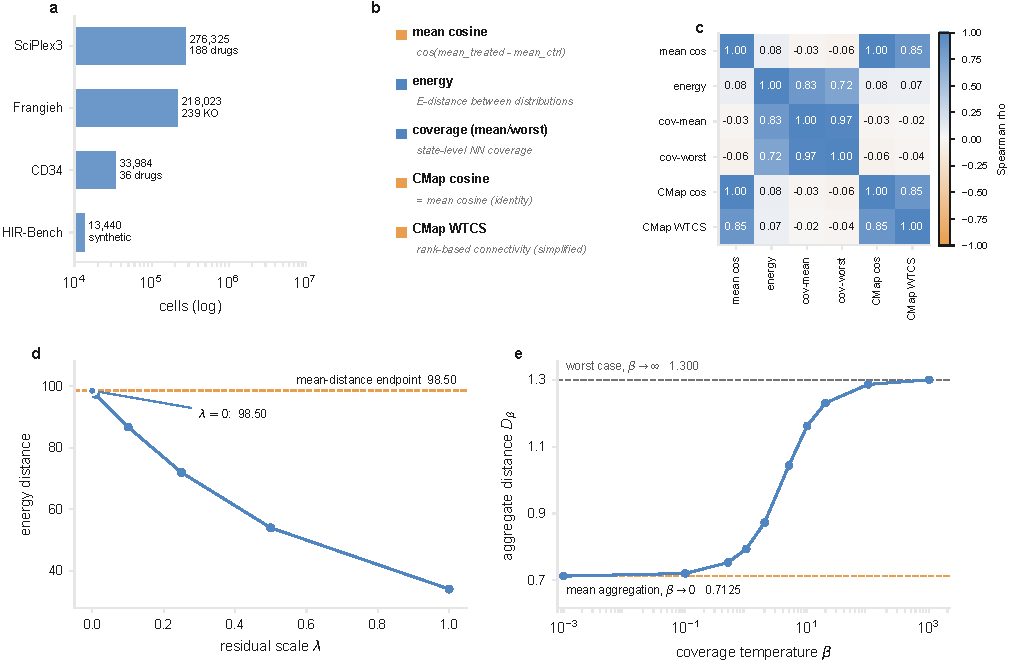
\includegraphics[width=\textwidth]{figures/edfig1.pdf}
\caption{\textbf{Reproducibility basis.} \textbf{a}, Dataset scale across the four benchmarks (cells, perturbations). \textbf{b}, Distributional metric-family definitions. \textbf{c}, Spearman correlation among all retrieval metrics, computed over the 54,180 query--candidate scores generated by 1,260 retrieval queries (43 candidates each; the unit is the scored pair, not the query): mean cosine and CMap cosine are perfectly correlated ($\rho=1.00$), while energy and coverage metrics form a separate, near-orthogonal block.}
\label{fig:ed1}
\end{figure}

\clearpage

% EXTENDED DATA FIGURE 2
\begin{figure}[htbp]
\centering
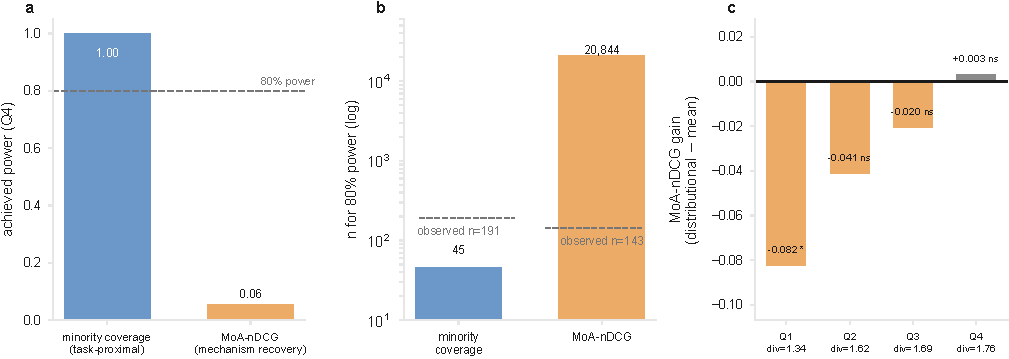
\includegraphics[width=\textwidth]{figures/edfig2.pdf}
\caption{\textbf{The Class B negative is not a power artifact.} \textbf{a}, Achieved power to detect the Q4 effect: the task-proximal minority-coverage metric is fully powered (1.00, n=191), the task-proximal MoA-nDCG is not (0.06, n=143). \textbf{b}, Sample size for 80\% power: 45 versus 20,844 queries. \textbf{c}, MoA-nDCG gain by divergence stratum. It is significantly \emph{negative} in Q1 (median $-$0.030, Benjamini--Hochberg $q=5.8\times10^{-5}$) and has a median of exactly zero in Q2--Q4, with no stratum showing a significant positive gain; the highest-divergence stratum's small positive \emph{mean} ($+0.003$) is not significant ($q=0.57$). MoA-nDCG is undefined for the leave-MoA-out and partial-library splits, where the mechanism class is removed from the library, so those 165 of 765 queries are excluded and n=600. A power deficit alone therefore does not explain the null: at the divergence level where the theory predicts the largest gain, the effect is absent, and where responses are least divergent it is adverse.}
\label{fig:ed2}
\end{figure}

\clearpage


% EXTENDED DATA FIGURE 3
\begin{figure}[p]
\centering
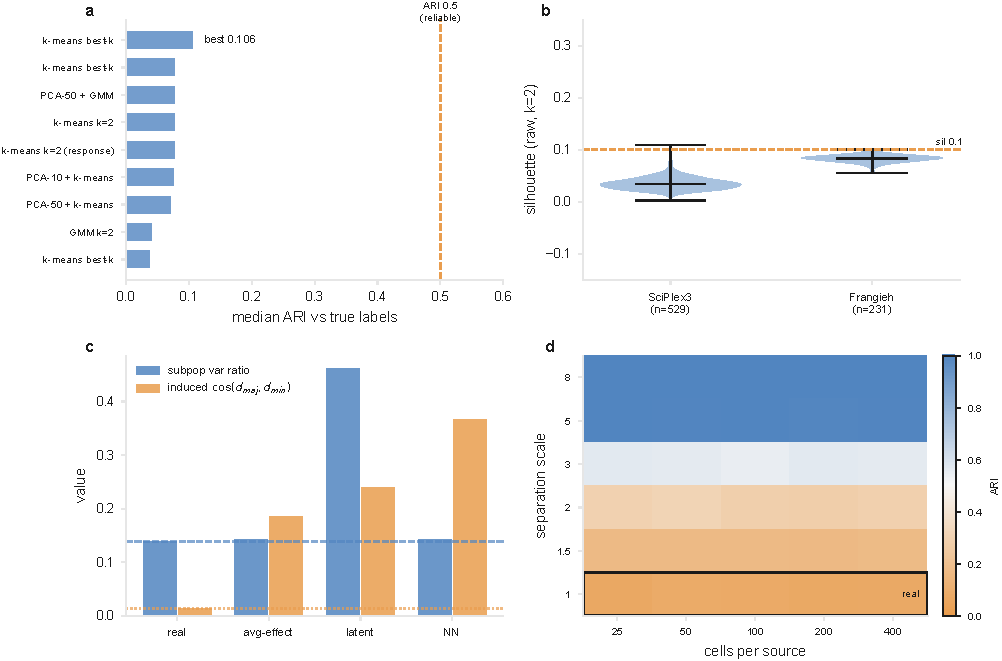
\includegraphics[width=\textwidth,height=0.30\textheight,keepaspectratio]{figures/edfig3.pdf}
\caption{\textbf{Subpopulation identifiability in the constructed mixture, and why this panel alone could not settle it.} \textbf{a}, The original nine-column clustering sweep on a known bimodal mixture, reported here for completeness and superseded by main-text Fig.~6e. The best value across methods is a median adjusted Rand index of 0.106, an \emph{upper bound} rather than a typical value: it is the best-case column taken over the minority of seeds in which that column wins, while the dense per-method columns lie at 0.037--0.078 and the global maximum over all methods and seeds is 0.149. The nine columns comprise only 6--7 \emph{distinct} algorithms (the response-space $k{=}2$ column is bit-identical to its raw-expression counterpart because $k$-means is translation-invariant, and the three best-$k$ columns are one method under three names), and \emph{all are centroid- or Gaussian-based}. \textbf{This panel alone cannot support the conclusion once drawn from it.} Clustering failure is consistent both with the information being absent and with its being present but unreachable without labels, and those have opposite implications. Main-text Fig.~6e resolves it by adding the graph- and density-based methods missing here (Leiden, HDBSCAN) and, decisively, a supervised ceiling: the ceiling is 0.692 accuracy and the best unsupervised method reaches 0.674, so \emph{within this constructed mixture} the limit is informational rather than algorithmic. \textbf{That qualifier turned out to be everything, and even the corrected reading was corrected again.} The 0.692 ceiling is largely an artefact of \emph{pooling} several HDAC and several JAK compounds into two classes: split the same cells one drug against one drug and the ceiling rises to 0.879. Posed as the same drug-response question in a patient's tumour, the ceiling is 0.923 while unsupervised clustering reaches only 0.777, a gap of $+0.117$ (main-text Fig.~5d): the information is present and the clustering step cannot reach it, so in real tissue the limit is \emph{algorithmic}, not informational. An intermediate version of this correction compared the drug-response partition here with a \emph{cell-type} partition in the tumour (malignant versus myeloid control cells, ceiling 0.964), which is a far easier question and licensed nothing; that number is withdrawn too. The general claim once drawn from this panel is withdrawn. \textbf{b}, Silhouette scores near zero in both datasets. The unit is the \emph{(cell line, drug) pair}, not the drug (529 SciPlex3 pairs from a 188-drug panel, 231 Frangieh; CORRECTIONS.md R29). Pooled median 0.040, and the two datasets differ: 0.034 for SciPlex3 against 0.084 for Frangieh. Only 0.4\% of pairs exceed 0.1 in either. Consistent with the constructed-mixture reading. \textbf{c}, Structure diagnostics for predicted versus real candidate populations. Predicted populations \emph{retain} baseline structure (subpopulation-variance ratio 0.142 versus 0.138 real); what they appear to lack is differential response (induced response cosine 0.19--0.37 versus 0.014 real). \textbf{That comparison does not survive scrutiny and is retained only for the structure-preservation point, which does not depend on it}: these candidate populations blend two cell lines, so an additive predictor emits a different delta per context, and for a latent model the response measured against real control cells is contaminated by the generator's reconstruction bias. Measured within one context and against the model's own baseline, an additive predictor returns exactly 1.000000 (main text; CORRECTIONS.md R28, R30). Predicted populations are synthesized by applying the predicted effect to the query context's real control cells; synthesizing them instead as an isotropic Gaussian around a single mean would make every structure diagnostic a measurement of the synthesizer (isotropy index 0.998, variance ratio 0.009 by construction), see Methods. \textbf{d}, Identifiability phase diagram over separation $\times$ cell budget: only source separation lifts ARI, and the cell-budget axis is flat, so the failure is not a sample-size problem. The separation manipulation is fit once on the full source populations, independently of the sample being evaluated; fitting it on the sampled cells and then shifting those same cells amplifies whatever separation each small draw happens to contain and yields the indefensible result that ARI \emph{falls} as the cell budget rises. See Methods.}
\label{fig:ed3}
\end{figure}

\clearpage

% EXTENDED DATA FIGURE 4
\begin{figure}[htbp]
\centering
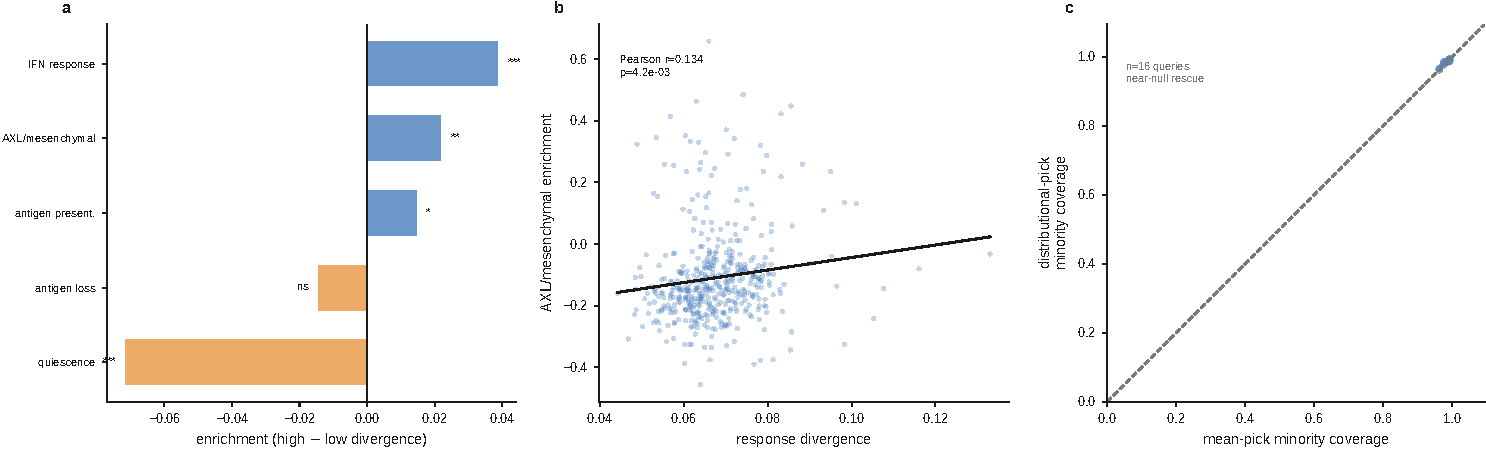
\includegraphics[width=\textwidth]{figures/edfig4.pdf}
\caption{\textbf{Exploratory resistance-associated divergence.} \textbf{a}, Program enrichment in high- versus low-divergence minority states (IFN response $p=1.9\times10^{-6}$, AXL/mesenchymal $p=3\times10^{-3}$). \textbf{The largest-magnitude effect in this panel is neither of those, and we do not interpret it.} The quiescence program carries an enrichment of $-0.072$, nearly twice the size of the next largest ($+0.039$ for IFN response), and it is highly significant on its face ($p = 7.7\times10^{-7}$, marked \textbf{***}). Its \emph{sign} is not stable across runs, so we report the bar rather than suppress it, and we draw no conclusion from it (Supplementary Note 3). Removing it because it is inconvenient would be the selection this paper exists to criticize; leaving it unlabelled would be worse. \textbf{b}, AXL/mesenchymal enrichment versus response divergence (Pearson $r=0.134$). \textbf{c}, Minority-rescue contrast between the distributional and mean picks is near null. All signals are exploratory and hypothesis-generating, with no survival or timecourse validation.}
\label{fig:ed4}
\end{figure}

\clearpage

% EXTENDED DATA FIGURE 5
\begin{figure}[htbp]
\centering

\includegraphics[width=\textwidth]{figures/edfig5.pdf}
\caption{\textbf{The absolute-potency confounder audit, and why it is not a Class-C result.} An earlier version of this work graded the retrieval rankings against \emph{absolute} drug potency and concluded that retrieval similarity is anti-aligned with therapeutic utility. That conclusion is withdrawn, and this figure records both the analysis and the reason. \textbf{a}, Scored against absolute GDSC2 AUC, every retrieval ranking inverts (energy $\rho=-0.52$; a mean baseline without control subtraction, $-0.53$; the correctly specified incumbent, $+0.10$) while a query-independent scalar that ranks candidates by the magnitude of their own response and never looks at the query reaches $+0.69$. \emph{The oracle is mismatched to the task.} A similarity retriever is asked which candidate resembles the query, not which kills hardest; handed a weak query it should correctly return other weak drugs, and this scoring counts that as failure. Because potency is largely driven by response magnitude, a magnitude scalar is near-guaranteed to win here. No therapeutic conclusion follows in either direction. The semantically matched oracle, drug--drug functional similarity, is in main-text Fig.~4h,i. \textbf{b}, What the audit does establish, and it is the reason the magnitude control is mandatory: the energy \emph{distance} between a query and a candidate is largely a function of the candidate's own response magnitude (median $\rho=+0.791$ across queries), because large-response populations sit far from everything. Ranking nearest-first therefore systematically returns the smallest-response candidates. Any distributional retrieval method claiming a functional validation must be shown to beat a scalar magnitude baseline.}
\label{fig:ed5}
\end{figure}

\clearpage

% EXTENDED DATA FIGURE 6
\begin{figure}[htbp]
\centering

\includegraphics[width=\textwidth]{figures/edfig6.pdf}
\caption{\textbf{HIR-Bench: the panels demoted from the main text.} Main-text Fig.~5 keeps only the two HIR-Bench panels that carry argument, the analytic condition under which subpopulation structure can change a decision and the $2\times2$ that \emph{measures} circularity. The four panels here were previously in the main text and should not have been: HIR-Bench's phase boundary is designed into its generator, so recovering it verifies that the benchmark works rather than establishing anything about biology, and its transfer to real data fails (Supplementary Note 1). A reader could reasonably have read four main-text panels of a synthetic benchmark as biological evidence. They are retained because they document that the benchmark behaves as specified, which is a precondition for trusting the two panels that stayed. \textbf{a}, Generative model: a query response is a majority plus a minority subpopulation with welfares A and B. \textbf{b}, Energy-minus-mean Hit@1 across the (minority fraction, conflict) grid. \textbf{c}, Best decision regret by information condition. Collapsing candidates to their means inflates regret against both objectives and most severely against the worst-welfare one (0.29 observed versus 0.96 predicted-mean), which is the objective that depends on the minority subpopulation. \textbf{d}, Benchmark sanity checks: the no-conflict flip rate is 0.000 and the median boundary margin 0.27, both within threshold.}
\label{fig:ed6}
\end{figure}

\clearpage

% EXTENDED DATA FIGURE 7
\begin{figure}[htbp]
\centering
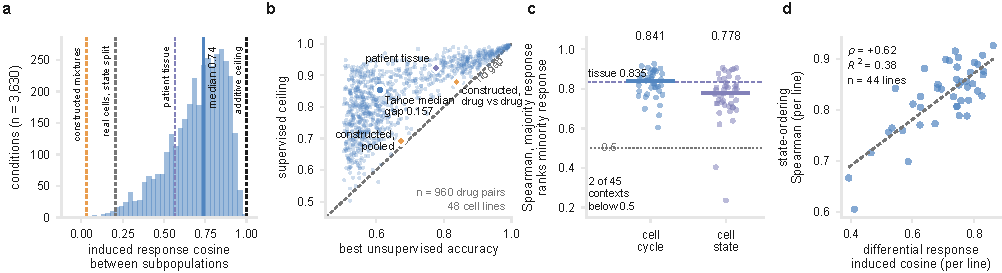
\includegraphics[width=\textwidth]{figures/edfig7.pdf}
\caption{\textbf{The two gates, and the premise statistic behind the proposed third, re-measured on unconstructed material.} Gate 3 is proposed rather than measured in this paper (main-text Fig.~6a and Results), and that status is unchanged here: panel \textbf{c} recomputes the statistic Gate 3 rests on, not decision relevance itself, since no candidate ranking and no decision outcome enter this dataset.
Tahoe-100M plate 3 (Zhang \emph{et al.} 2025; \texttt{10.1101/2025.02.20.639398}): a complete grid of 50 cancer cell lines against 93 compounds at one
dose, a vehicle arm in every line, 4,158,278 cells, median 648 cells per condition. Its
within-line heterogeneity is intrinsic cell state, not two populations combined by us, which is
the property that makes it useful here. \textbf{It is not tissue, and it is used for sample size
rather than for relevance}; the paper's claims about what matters therapeutically continue to rest
on the patient data of main-text Fig.~5. The statistics are the paper's own, not new ones.
\textbf{a}, Gate 1. Induced response cosine between the two subpopulations of a treated population,
each referred to its own matched control, over 3{,}630 conditions
(median 0.739). Dashed lines mark the four values the main text quotes.
Our constructed mixtures are not at one end of the unconstructed range: only
0.11\% of conditions are as divergent as they are. \textbf{b}, Gate 2,
posed as the same drug-response question and scored with the same four-method clusterer panel.
One point per drug pair; diamonds are the three main-text settings. Supervised ceiling
0.853 against best unsupervised 0.611,
a gap of 0.157 that is positive in 48
of 48 cell lines. No method family rescues it (k-means
0.592, Gaussian mixtures 0.582, Leiden
0.563), which differs from the tumour, where Leiden was the method that
partly survived. \textbf{c}, Gate 3 under two partitions, both computed on \emph{disjoint} cell
sets, against the tumour value computed the same way (0.835). Medians
0.841 and 0.778. The condition is not
universal: 2 of 45 contexts fall
below 0.5 under the control-state partition, the lowest at 0.236, and
those are the contexts in which a distributional score should pay off. \textbf{d}, Gate 3 against
Gate 1 within the cell-cycle partition, which is the only comparison of the two that is
like-for-like. They share some variance and are not the same condition. \textbf{Limits.} These are
cell lines; this is one plate of fourteen and 93 of 380 compounds; both partitions are coarse
two-way splits of cell state rather than the persister axis that motivates the paper; and which
contexts show an open Gate 3 depends on the partition, the two agreeing at the extremes but only
moderately in rank (Spearman 0.466).}
\label{fig:ed7}
\end{figure}

\clearpage

%% =====================================================================
%%  SUPPLEMENTARY NOTES
%% =====================================================================

\noindent{\large\textbf{Supplementary Note 1. HIR-Bench: sanity checks, and why the transfer
test's 100\% flag rate is not evidence.}}
\bigskip

\noindent The benchmark's internal checks hold on the full grid: the no-conflict flip rate is
0.0000, as it must be for a generator whose flip boundary is $\alpha^* = B/(A+B)$, and the median
boundary margin is 0.27.

Under the information-condition transfer test, the gate flags mean-collapsed predicted responses
as no-distributional in 100\% of cases. We decline to count that number as evidence, because it is
a \textbf{tautology}: the rule returns no-distributional \emph{unconditionally} whenever the
information condition is predicted-mean. It cannot return anything else, so the 100\%
restates the rule rather than testing it. The substantive claim, that mean-collapsed candidate
libraries offer no distributional advantage, rests on the predict-then-rank experiments of the main
text, not on this figure.

The projection of the HIR-Bench regime boundary onto real data \textbf{fails its own acceptance
test, and we report it as failing}. The label is heavily imbalanced (228 to 11), so a constant
predictor scores 95.4\%; the regime projection scores 61.1\%, which is 34 points \emph{worse} than
saying nothing. The boundary does not transfer. Two structural limits bound the test in both
directions and we work around neither: the boundary is fitted on the method-performance layer,
which is available on a 144-instance grid (72 grid cells) because scoring nine retrieval methods
against up to 100 candidates per instance does not scale to the full grid; and the acceptance
label derives from the same uncalibrated $+0.01$ threshold the main text declines to trust.

\bigskip
\noindent{\large\textbf{Supplementary Note 2. Two further tests of the two-gate criterion.}}
\bigskip

\noindent \textbf{(a) Coverage performance versus query identifiability.} The two gates predict
where a subpopulation-coverage score should and should not carry signal. Stratifying real-data
coverage by query identifiability is consistent with them, but weakly and \emph{not}
monotonically. Coverage MoA-nDCG is higher for more identifiable queries (Spearman $\rho = 0.17$,
$p = 6.3\times10^{-5}$, $n = 543$ query-seed pairs), but the lift is confined to the top tertile:
tertile means are 0.285, 0.240 and 0.444 from least to most identifiable, so the middle tertile
sits \emph{below} the least-identifiable one. Two caveats bound even that. The most-identifiable
tertile carries a median of 6 same-mechanism candidates against 2 in the other two tertiles, and a
larger positive pool mechanically raises nDCG, so the correlation is not cleanly separated from
candidate-pool size. And Gate 2 is almost never open \emph{in these SciPlex3 queries}: even the
most-identifiable tertile has a median silhouette of 0.038. That scope matters. On patient
glioblastoma the same gate is wide open (main-text Fig.~5d), so the statement here is a fact about
the cell-line data this note analyses and not about biology.

\textbf{(b) The conditional advantage the criterion predicts is absent.} If identifiable structure
is what lets distributional scores help, the per-query mechanism-recovery advantage should turn
positive where structure is present. Stratifying 600 leave-drug-out queries by response divergence,
it does rise, and the ordering is real and leakage-free (Spearman $\rho = 0.14$, permutation
$p = 2\times10^{-4}$). But it never clears parity: the most-divergent stratum reaches only $+0.02$
in nDCG, with a bootstrap interval spanning zero, and it reverses in one of three cell lines.
Decisively, when queries are stratified by the actual Gate-2 variable, query identifiability
(silhouette), the advantage is flat ($\rho \approx 0$). Response divergence measures response
spread, not resolvable subpopulation structure, and Gate 2 does not open \emph{in these SciPlex3
queries} even for the most response-divergent ones. \textbf{This is not a statement about real
tissue}, and an earlier version of this note wrote it as though it were. On patient glioblastoma
Gate 2 opens (main-text Fig.~5d) and the mechanism a distributional advantage would run through is
nonetheless largely absent; no retrieval was run on that cohort, so no advantage was measured there
either way. Together with the SciPlex3 stratification above, that is why the two-gate criterion is
reported as necessary but not sufficient.

\bigskip
\noindent{\large\textbf{Supplementary Note 3. Exploratory resistance-associated divergence.}}
\bigskip

\noindent In the Frangieh melanoma Perturb-CITE-seq data, cells whose response direction diverges
most between immune contexts are enriched for resistance-associated programs: an AXL/mesenchymal
program (correlation $+0.134$, $p = 0.003$), an interferon-response program
($p = 1.9\times10^{-6}$), and antigen-presentation genes ($p = 0.04$); see Extended Data Fig.~4.

This analysis is \textbf{exploratory and hypothesis-generating throughout} and is reported as a
direction for future work, not as a result. There is no longitudinal drug timecourse, no survival
readout, and no post-treatment clone measurement, so we make \textbf{no claim that a distributional
score predicts resistance} or identifies persister cells. A quiescence program's sign was not
stable across runs and is not interpreted. Consistent with the rest of the study, the
distributional-versus-mean minority-rescue contrast is itself near-null. The observation motivates
future experiments with functional readouts, and nothing more.

\clearpage

% SUPPLEMENTARY TABLE 1
\renewcommand{\thetable}{S\arabic{table}}
\setcounter{table}{0}

\noindent{\large\textbf{Supplementary Table 1. Datasets, preprocessing, and query construction.}}
\bigskip

\noindent\textbf{(a) Dataset scale.} Four benchmarks span controlled proof, natural heterogeneity, an honest negative control, and a synthetic analytic stress test.

\begin{table}[htbp]
\centering
\small
\begin{tabular}{@{}lrlll@{}}
\toprule
Dataset & Cells & Genes & Context axis & Perturbations \\
\midrule
SciPlex3 (Srivatsan 2020)          & 276{,}325 & 2{,}000 HVG & A549, K562, MCF7                & 188 drugs (all 3 lines) \\
Frangieh (2021)          & 218{,}023 & 2{,}000 HVG & Control, IFN$\gamma$, Co-culture & 239 CRISPR KOs \\
CD34$+$ (GSE306429)                   & 33{,}984  & 2{,}000 HVG & discovered subpopulations       & 36 drugs \\
HIR-Bench (synthetic instances)       & 13{,}440  & latent      & two-subpopulation welfare model & tunable conflict \\
GDSC2 dose-response (Class C)         & \multicolumn{2}{l}{286 drugs $\times$ 969 lines} & 966 lines (SciPlex3 lines held out) & 35 matched compounds \\
Tahoe-100M plate 3 (Zhang 2025)       & 4{,}158{,}278 & 2{,}304 HVG & 50 cancer cell lines & 93 compounds, 1 dose \\
\bottomrule
\end{tabular}
\end{table}

\noindent\textbf{(b) Preprocessing.} Processed tensors are built once and read directly by the retrieval code; the build scripts are kept for provenance.

\begin{table}[htbp]
\centering
\small
\begin{tabular}{@{}ll@{}}
\toprule
Step & Setting \\
\midrule
Source & SciPlex3: Srivatsan \& Trapnell 2020; Frangieh: scPerturb Zenodo; CD34$+$: GSE306429 counts layer \\
Normalization & log-normalized expression; 2{,}000 highly variable genes selected per dataset \\
Controls & real DMSO controls (SciPlex3); condition controls (Frangieh); DMSO (CD34$+$) \\
Response delta & per-cell expression minus matched control centroid, used only where a metric requires it \\
Dose & 10{,}000 nM (SciPlex3 controlled and cross-line experiments) \\
\bottomrule
\end{tabular}
\end{table}

\noindent\textbf{(c) Query construction.} A query is a mixture of two response modes at mixing weight $\alpha$; the retrieval task is to rank the candidate that generated it above distractors.

\begin{table}[htbp]
\centering
\small
\begin{tabular}{@{}lll@{}}
\toprule
Parameter & Controlled (SciPlex3) & Cross-line / natural \\
\midrule
Response modes            & HDAC (class a) vs JAK (class b) & cell-line pairs / immune-context pairs \\
Query size                & 400 cells                       & 200 cells \\
Distractors               & 40                              & 40 \\
Mixing weight $\alpha$    & 0.5, 0.6, 0.7, 0.8, 0.9         & 0.5--0.9 \\
Seeds                     & 20 (base 1000)                  & 10 (cross-line), 20 (Frangieh) \\
Identifiability probe     & min 30 cells, gate 0.9          & min 30--40 cells, gate 0.9 \\
\bottomrule
\end{tabular}
\end{table}

\noindent\footnotesize Cell and gene counts are the processed-tensor totals. HIR-Bench's 13{,}440 entries are synthetic benchmark \emph{instances} (672 parameter configurations $\times$ 20 seeds), not biological cells; they are the grid used for the predictability analysis (main-text Fig.~5b).
\normalsize

\clearpage

% SUPPLEMENTARY TABLE 2
\noindent{\large\textbf{Supplementary Table 2. Field-level evaluation audit.}}
\bigskip

\noindent The claim that objective-aligned evaluation is a field-wide default should be checkable rather than asserted, so the audit is reproduced here rather than left with the code. \textbf{Inclusion criteria:} a method family qualifies if (i) it ranks or selects perturbations, or predicts perturbation responses that a ranking layer consumes, (ii) it is represented by at least one widely used published implementation, and (iii) its headline evaluation metric is stated in the source. \textbf{Alignment} is judged \emph{high} when the headline metric is a monotone transform of the scoring rule's own objective evaluated on the same data, which is the condition under which a gain is close to guaranteed. Families are the unit; we do not score individual papers, and this is an audit of \emph{evaluation practice}, not of correctness.

\begin{table}[htbp]
\centering
\footnotesize
\renewcommand{\arraystretch}{1.25}
\begin{tabular}{@{}p{2.5cm}p{3.0cm}p{2.9cm}p{3.0cm}p{1.2cm}p{2.1cm}@{}}
\toprule
Method family & Representative methods & Objective & Headline evaluation & Metric class & Alignment risk \\
\midrule
CMap / L1000 signature retrieval & Connectivity Map (Lamb \emph{et al.} 2006); L1000 / WTCS connectivity (Subramanian \emph{et al.} 2017) & rank by connectivity of mean differential signatures & connectivity score; cosine of mean signatures & A & high: the metric is the scoring rule restated \\
Single-cell signature retrieval & pseudobulk and single-cell connectivity on harmonized perturbation atlases (Peidli \emph{et al.} 2024) & rank by single-cell-derived mean or pseudobulk signature match & signature correlation; Hit@$k$; DEG overlap & A (B via DEG) & high: signature-space metric mirrors signature-space scoring \\
Distributional retrieval (\textbf{this work}) & energy, MMD, sliced-Wasserstein, subpopulation coverage & rank by population-to-population distributional distance & energy/MMD welfare-regret proxy (A); MoA-nDCG, minority coverage (B); GDSC functional similarity (C) & A + B + C & high on the Class-A proxy; \emph{self-raised and measured here} \\
Single-cell perturbation predictors & scGen (Lotfollahi \emph{et al.} 2019); CPA (Lotfollahi \emph{et al.} 2023); chemCPA (Hetzel \emph{et al.} 2022) & predict post-perturbation expression from control & reconstruction MSE / $R^2$ / PCC of predicted delta & A (B via DEG) & high: training loss and evaluation share the reconstruction target \\
Virtual-cell / perturbation foundation models & scGPT (Cui \emph{et al.} 2024); scFoundation (Hao \emph{et al.} 2024); Geneformer (Theodoris \emph{et al.} 2023) & general-purpose prediction of perturbed cell state & held-out reconstruction; embedding similarity & A + B & high: reconstruction and embedding metrics align with the pretraining objective \\
Graph / target-based inverse design & GEARS (Roohani \emph{et al.} 2024); network-proximity repositioning (Guney \emph{et al.} 2016) & rank by graph proximity or target overlap & graph proximity; target-family overlap & A & high: the scoring graph and the evaluation graph coincide \\
Target/drug graph methods (PDGrapher-style) & PDGrapher (Gonzalez \emph{et al.} 2026) & predict interventions moving a cell state toward a target & closed-loop target ranking recall/nDCG & A (B via target family) & high: the closed-loop metric is aligned with the graph objective \\
\bottomrule
\end{tabular}
\end{table}

\noindent\footnotesize The table audits \textbf{six published method families}, with the present work listed as a seventh row for contrast and excluded from every count below. Each of the six published families has a headline metric in Class A, and none reports a Class-C readout as its primary evidence. This is the pattern the present study raises against itself: we report all three classes on one task set, and the Class-A gain does not survive the other two at anything near its apparent size. The unit of the audit is the \emph{family}, not the paper, and it is an audit of evaluation practice rather than of correctness; we do not score individual papers. The \textbf{representative methods} column names widely used implementations so that each row can be checked against specific work rather than taken on assertion; being named there is not a criticism of a method, and the objective and headline-evaluation columns describe the family's common practice rather than any one paper's full evaluation. Full citations with DOIs accompany the code.
\normalsize

\clearpage

% SUPPLEMENTARY TABLE 3
\noindent{\large\textbf{Supplementary Table 3. Cell-compartment validation in the natural-heterogeneity benchmark.}}
\bigskip

\noindent The natural-heterogeneity result (main-text Fig.~5d--f) depends entirely on the cell-type labels being what they claim to be, so the labelling is validated rather than trusted. Each cell receives a $z$-scored marker score per compartment and is called only if it scores highest for that compartment, clears an absolute expression floor on that compartment's key markers, and beats the runner-up by a margin; everything else is labelled unassigned and \emph{dropped} (39.9\% of cells). The table below reports, for each called compartment, the mean log-normalized expression of every compartment's key marker set. A compartment passes only if its own markers are the most strongly expressed. The loader raises rather than writing labels if any compartment fails.

\begin{table}[htbp]
\centering
\small
\begin{tabular}{@{}lrrrrc@{}}
\toprule
Called compartment & Cells & \multicolumn{3}{c}{Mean expression of key markers for} & Passes \\
\cmidrule(lr){3-5}
 & & malignant & myeloid & oligodendrocyte & \\
\midrule
Malignant glioma      & 41{,}314 & \textbf{1.024} & 0.073 & 0.117 & yes \\
Tumour-assoc. myeloid & 31{,}678 & 0.121 & \textbf{1.534} & 0.169 & yes \\
Oligodendrocyte       & 23{,}233 & 0.409 & 0.114 & \textbf{1.784} & yes \\
\bottomrule
\end{tabular}
\end{table}

\noindent\footnotesize \textbf{What this table exists to prevent.} A first version of the assignment took a bare argmax over five marker sets, which forces every cell into some compartment, including cells expressing none of the markers. It produced two compartments that fail exactly this check: cells labelled T cells (22\% of the dataset) had a mean CD3D/CD3E/CD2 expression of 0.080, \emph{lower} than their malignant-marker score of 0.141, and cells labelled endothelial expressed myeloid markers (1.074) more strongly than endothelial ones (0.951). They were neither. Building a natural-heterogeneity result on a fabricated T-cell compartment would have been worse than reporting no natural dataset at all, and only the three compartments above are used.
\normalsize

\clearpage

% SUPPLEMENTARY TABLE 4
\noindent{\large\textbf{Supplementary Table 4. The Class-C functional oracle, under both constructions.}}
\bigskip

\noindent Cell lines differ greatly in general drug sensitivity, and that shared main effect inflates every drug--drug correlation: left uncorrected, 85\% of drug pairs appear positively similar (median $+0.178$). The oracle used in the main text therefore subtracts each cell line's mean AUC, estimated across all 286 GDSC2 compounds, before correlating; the corrected oracle is symmetric about zero (52\% positive, median $+0.015$). \textbf{That choice decides the result, and the table below is why we state the dependence in the main text rather than reporting only the ordering we prefer.} Values are median per-query Spearman $\rho$ against the oracle, over 103 leave-one-drug-out queries in three cell lines.

\begin{table}[htbp]
\centering
\small
\begin{tabular}{@{}lcc@{}}
\toprule
Ranking rule & Corrected oracle & Uncorrected oracle \\
 & (cell-line mean removed) & (raw AUC profiles) \\
\midrule
Energy distance (the distributional score)      & \textbf{+0.276} & +0.097 \\
Mean cosine, control-subtracted (the incumbent) & +0.083 & \textbf{+0.138} \\
Mean cosine, no control subtraction             & +0.241 & +0.092 \\
Magnitude matching (query-dependent scalar)     & +0.232 & \textbf{+0.217} \\
Magnitude only (query-independent)              & $-$0.330 & +0.135 \\
Potency matching (diagnostic, not a recommender)& +0.399 & +0.290 \\
\midrule
Energy, partialled on magnitude matching        & +0.097 & n/a \\
\bottomrule
\end{tabular}
\end{table}

\noindent\footnotesize \textbf{What flips and what does not.} Under the corrected oracle the distributional score leads its incumbent threefold ($+0.276$ against $+0.083$), and that is the one criterion in this study, invisible to every scorer, on which it wins. Under the uncorrected oracle it does not win at all: energy falls to $+0.097$, \emph{below} the incumbent's $+0.138$ and well below the magnitude scalar's $+0.217$. The affirmative Class-C finding is therefore conditional on the centering. We think the centering is right, we specified it on the reasoning above before inspecting any retrieval result, and leaving a shared cell-line main effect inside an oracle would be an error in its own right. But a paper whose thesis is that the choice of criterion decides the winner cannot quietly exempt its own criterion, and an earlier draft of this work asserted that both oracles ``give the same verdict'', which the table shows is false. \textbf{What survives both constructions is the negative result}: under neither oracle does the distributional score significantly beat a scalar that compares no distributions at all. Note also that energy's uncorrected value ($+0.097$) and its magnitude-partialled value under the corrected oracle ($+0.097$) coincide to three decimals by arithmetic accident; they are different quantities ($0.0967$ and $0.0969$ before rounding).
\normalsize

\clearpage

\clearpage
\noindent{\large\textbf{Supplementary Note 4. What this study does not claim.}}
\medskip

\noindent This note states the scope of every claim in the main text. It is reproduced in full from
an earlier main-text box and is referenced from the Discussion.
\medskip

\begin{enumerate}[leftmargin=1.4em,itemsep=1pt,topsep=1pt]
\item \textbf{We do not claim that the predictors tested here represent the field.} The in-repository linear-latent model (PCA encoder, additive latent delta, linear decoder) is additive \emph{by construction}, so its Gate-1 value demonstrates an algebraic property rather than surveying deployed models. We \emph{do} now report one deployed model: the published scGen variational autoencoder passes its learning check and returns a true induced divergence of 0.972 against an additive ceiling of 1.000, so it is near-additive in practice. That is one model, not a field.
\item \textbf{We show that a non-additive predictor opens Gate 1, but not that opening it buys retrieval gain, and the second half is the experiment that would falsify us.} A latent-space entropic optimal-transport map passes its learning check ($0.352$) and reaches a true induced divergence of $0.900$, significantly below the additive ceiling of $1$, so Gate 1 does open; but only a crack, since real cells sit at $0.205$, and the map's learning is weak. The same map run naively in gene space did not clear the bar (learning $0.057$), and the published CPA model, though it reconstructs cells at $R^2\approx0.39$, does not learn per-drug effects at either sixty or three hundred cells per drug (delta learning $0.08$ in both) and is therefore void. We did re-run the predict-then-rank retrieval with this Gate-1-opening map, and it was inconclusive: the OT map's cross-line predictions are too poor to retrieve with at all (Hit@1 $0.05$ under every rule, against $0.88$ for the additive predictor), so we lack a predictor that both predicts accurately and opens Gate 1, and whether opening Gate 1 buys a distributional advantage stays untested. A modern flow-matching model, CellFlow, conditioned on ECFP4 compound fingerprints, learns within context (mean-delta cosine $0.24$, opening Gate 1 at induced divergence $0.85$) but collapses to $0.03$ under leave-one-context-out at a matched budget, an $8.4\times$ drop; per drug this transfer tracks cross-context response similarity ($r = 0.85$), so it too cannot serve as the clean cross-context predictor the falsification requires. The collapse holds under distributional (energy) and differential-expression metrics, not only the mean-delta check; and conditioning CPA on the same ECFP fingerprints instead of a learned embedding does not rescue it (learning $0.03$), locating that failure in the adversarial objective rather than the drug representation.
\item \textbf{We do not claim that the distributional score provides better therapeutic recommendations.} Every gain in this study is measured under an objective-aligned (Class A), task-proximal (Class B), or semi-real functional (Class C) criterion. None is a clinical or same-cell endpoint.
\item \textbf{We do not claim that the functional-oracle advantage is a distributional effect, nor that it is robust to how the oracle is built.} Energy retrieval does beat the correctly specified mean incumbent under the cell-line-centred GDSC oracle ($+0.276$ versus $+0.083$), but a query-dependent scalar that compares no distributions reaches $+0.232$, energy beats it on only 62 of 103 queries ($p = 0.073$, itself anticonservative), and partialling that magnitude channel out leaves $+0.097$: the gain is real and mostly not distributional. It is also conditional on the centering, since under the uncorrected oracle energy falls to $+0.097$ and loses to both the mean incumbent ($+0.138$) and the scalar (Supplementary Table 4). We specified the centering in advance and argue it is correct, but only the negative survives both constructions: under neither oracle does the distributional score significantly beat a scalar that compares no distributions.
\item \textbf{We do not claim that retrieval similarity is anti-aligned with therapeutic utility.} An earlier framing of this work graded the rankings against \emph{absolute potency} and drew that conclusion. It does not follow: a similarity retriever handed a weak query should return other weak drugs, and potency is largely driven by response magnitude, so a magnitude scalar is near-guaranteed to win that comparison. The absolute-potency analysis is retained only as a confounder audit exposing the magnitude channel.
\item \textbf{We do not claim an improvement under the task-proximal metric.} On the same scorer and the same queries that earn a Class-A gain of $+0.129$ (median), the mechanism-recovery gain is $0.000$ (median) and $-$0.037 (mean). Across 239 real-data tasks the coverage advantage is statistically real and negligible (mean $+0.0018$) and lives only in constructed cell-line mixtures.
\item \textbf{We do not report a count of ``distributionally dominant'' real tasks, and no such count should be quoted from this work.} The conventional threshold sits inside the noise band of the difference distribution, and the seed re-draws which drugs are tested and re-clusters the minority subpopulation, so it is not a replicate. Under resampling only 2 of the 10 threshold-crossing cross-line tasks survive, while drugs that cross the threshold at no seed in the recorded run cross it in \CONTROLRANGE{} of 10 resamples.
\item \textbf{We do not claim that HDAC inhibitors are a validated regime for distributional retrieval.} Exactly two tasks survive seed resampling, both HDAC inhibitors in one cell-line pair. With $n = 2$ that is a hypothesis, not a result.
\item \textbf{We do not claim that minority-state coverage is oracle-independent.} It is a mean-based cosine proxy and is not the distributional score's own objective, but it rewards covering the minority state, which is what the worst-case coverage scorer optimizes. It is task-proximal, not independent. Of the judges used here, MoA recovery is annotation-derived and the GDSC functional oracle is the only externally grounded one; the distributional score is worse than the incumbent on the first and better on the second, by a margin a scalar reproduces.
\item \textbf{We do not claim that the current gate reliably transfers to real retrieval tasks.} The gate is experimental; it does not isolate oracle-independent gains in partial-observed real data, its reliability axis is anti-correlated with true divergence ($\rho = -0.21$), and the dataset-level divergence criterion admits our negative control (CD34$+$, cosine 0.186) just as readily as our positive anchor. Its apparent success at flagging mean-collapsed predicted responses is a tautology: the rule returns no-distributional unconditionally for that information condition.
\item \textbf{We do not claim that HIR-Bench is a biological ground truth.} It is a constructive synthetic benchmark whose phase boundary is expected by design.
\item \textbf{We do not claim that subpopulation identifiability is an information limit, and we do not claim the opposite either.} Both readings appeared in earlier drafts and both are withdrawn. The first came from a constructed mixture that pooled several drugs into each class, which lowered its ceiling for reasons unrelated to biology. The second came from comparing that drug-response partition with a \emph{cell-type} partition in a tumour, which is an easier question and returned a reassuring 0.964 that meant nothing. Posed as the same question in both settings, the tumour ceiling is 0.923 and unsupervised clustering reaches 0.777: the information is present and the clustering step cannot reach it, so in real tissue the limit is algorithmic. That result rests on 4 patients, 30 of its 36 splits from one of them, and a compartment assignment that discards 39.9\% of cells, and it should be treated accordingly.
\item \textbf{We do not claim that our structure-preservation and induced-divergence diagnostics measure the perturbation rather than the generator.} A latent predictor returns $P(C) + W\delta_z$, the autoencoder's reconstruction plus the decoded delta. Referred to its own decoded baseline, an additive latent model induces \emph{exactly zero} response divergence ($\cos = 1.000000$). Referred to the \emph{real} control cells, which is what any retrieval scorer does, the same model shows apparent divergence as low as $-0.13$, and every bit of it is reconstruction bias. Our subpopulation-variance-ratio and induced-cosine diagnostics are computed against real controls and therefore inherit this contamination. We report both baselines and flag the affected numbers rather than quietly choosing the flattering one.
\item \textbf{We do not claim that the distributional score is better on the surface-protein oracle, nor that the mean is.} The winner is determined by whether that oracle is built as a mean or as a distribution, from the same proteins in the same cells. We report the reversal, not a victor. What the reversal does establish is that objective alignment is not confined to a method grading its own objective: it operates between external, blind criteria, and it therefore threatens external validations too, including ours.
\item \textbf{We do not claim that the distributional score predicts resistance.} The resistance analysis is exploratory and hypothesis-generating; there is no timecourse or survival readout, and the minority-rescue contrast is near-null.
\item \textbf{We do not benchmark live PDGrapher, and no number in this paper derives from LINCS.} Perturbation predictors are treated as candidate-response sources, not as models under test.
\item \textbf{We do not claim that all CMap implementations are algebraically identical to the score implemented here;} the exact identity is limited to the implemented cosine mean-signature kernel.
\end{enumerate}

\clearpage

\end{document}
